% Final report: Text- and Night-Light-Guided Satellite Embeddings for Regional Economic Estimation
% Build:  cd reports && latexmk -pdf final_report.tex      (figures from reports/figures, tables from reports/tables)
\documentclass[11pt,a4paper]{article}
\usepackage[T1]{fontenc}
\usepackage[utf8]{inputenc}
\usepackage{lmodern,microtype}
\usepackage[margin=2.3cm]{geometry}
\usepackage{amsmath,amssymb}
\usepackage{graphicx,booktabs,tabularx,multirow,array}
\usepackage[font=small,labelfont=bf]{caption}
\usepackage{subcaption}
\usepackage{xcolor}
\usepackage{tikz}
\usetikzlibrary{arrows.meta,positioning}
\usepackage{enumitem}
\usepackage[hidelinks]{hyperref}
\graphicspath{{figures/}{../presentation/midterm/assets/}}
\setlist{itemsep=2pt,topsep=4pt}
\newcommand{\R}{R\textsuperscript{2}}
\newcolumntype{L}{>{\raggedright\arraybackslash}X}
\renewcommand{\topfraction}{0.9}\renewcommand{\bottomfraction}{0.8}
\renewcommand{\textfraction}{0.07}\renewcommand{\floatpagefraction}{0.75}
\setcounter{topnumber}{3}\setcounter{bottomnumber}{2}\setcounter{totalnumber}{5}

\title{\textbf{Reading the Economy from Space}\\[4pt]
\large Text- and Night-Light-Guided Satellite Embeddings for Municipal GDP in Minas Gerais, Brazil}
\author{Group 2: Hemant (22CS30029), Saras Dipak Wagh (22CS30048), Pallav Agarwal (22CS30040)\\[2pt]
\small Term project, Geospatial Reasoning using LLMs and Generative AI \quad$\cdot$\quad
\href{https://github.com/chadsaras/GIS_Project}{github.com/chadsaras/GIS\_Project}}
\date{October 2026}

\begin{document}
\maketitle

\begin{abstract}
\noindent
We estimate 2022 GDP per capita for all 853 municipalities of Minas Gerais, Brazil, from free satellite data on a
1\,km grid (575{,}166 cells). The pipeline combines two recent ideas that had not been tested together: aligning
Google's frozen satellite embeddings (GSED) with text written by a vision--language model (as in UrbanCLIP), and
steering the embeddings towards economic activity with VIIRS night lights (as in Yue, Zhao and Hu, 2026).
Cell outputs are pooled to municipalities and trained on official IBGE GDP. Every number is out-of-sample under
5-fold spatial cross-validation over IBGE's 70 immediate regions, with all three learning stages retrained in each
round. The best model, a validation-chosen blend of the best embedding model with the night-light benchmark,
reaches \R{} 0.52 (RMSE 0.41 in log GDP per capita), against 0.27 (0.51) for night lights alone and 0.39 (0.47) for
LightGBM on the same embeddings. Adding captions gives the largest single gain (RMSE $-0.025$, 95\% block-bootstrap
interval $[-0.050, +0.004]$), but none of the four planned comparisons (night-light steering, text, POIs and roads,
hybrid) is significant. The largest errors are mining and steel municipalities, where a few cells produce most of
the output, and small public-sector towns. A blind audit of 300 captions finds a false claim in 35\% of raw
captions and 23\% after our data-based cleaning.
\end{abstract}

%=====================================================================
\section{Introduction}

Official GDP below the national level is often late, estimated from partial data, or missing. Satellites observe
every place with the same instruments every year, so a model that reads economic activity from satellite data gives
an independent and cheap estimate for every district. Two lines of recent work point in different directions.
\emph{UrbanCLIP} (Yan et al., 2024) generates a caption for every satellite tile with a vision--language model and
aligns image and text, reporting gains on urban indicators. \emph{Estimating Economic Activity from Satellite
Embeddings} (Yue, Zhao and Hu, 2026) starts from Google's 64-dimensional annual satellite embeddings and steers them
with night lights before aggregating to regions.

This project combines both in one pipeline and tests each ingredient under a strict spatial split. We ask five
research questions:
\begin{description}[leftmargin=1.2cm,style=nextline]
\item[RQ1] Does night-light steering improve municipal GDP estimates from satellite embeddings?
\item[RQ2] Does aligning the embeddings with generated text (captions plus data-derived fact sentences) help on top of steering?
\item[RQ3] Do points of interest and road lengths add information on top of text and steering?
\item[RQ4] Does a hybrid with the night-light benchmark beat the best single model?
\item[RQ5] Where and why does the best model fail?
\end{description}

\paragraph{Contributions.} (i) A reproducible 1\,km dataset for Minas Gerais joining GSED, VIIRS, ESA WorldCover,
OpenStreetMap, Microsoft building footprints, 10{,}000 captioned Esri tiles and IBGE statistics. (ii) An ablation of
twelve model variants on identical spatial folds, with block-bootstrap intervals for each research question.
(iii) A caption-cleaning step that checks generated sentences against map data, and a blind audit of its effect.
(iv) An error analysis that identifies where satellite data cannot see the economy.

%=====================================================================
\section{Study area and data}

\paragraph{Why Minas Gerais.} Brazil's statistics office IBGE publishes GDP for every municipality, and the 2022
Census gives exact population counts. Minas Gerais has 853 municipalities, far above the 150-unit minimum of the
proposal, and one of the widest income ranges in the country: GDP per capita runs from R\$\,8{,}049 in São João das
Missões (Jequitinhonha--north) to R\$\,390{,}991 in Catas Altas (an iron-mining town), a ratio of 49. The target is
$\log(\text{GDP}/\text{population})$, with mean 10.14 and standard deviation 0.60; on this scale an error of 0.1 is
about 10\%. Figure~\ref{fig:labels} shows its distribution and map.

\begin{figure}[!htbp]
\centering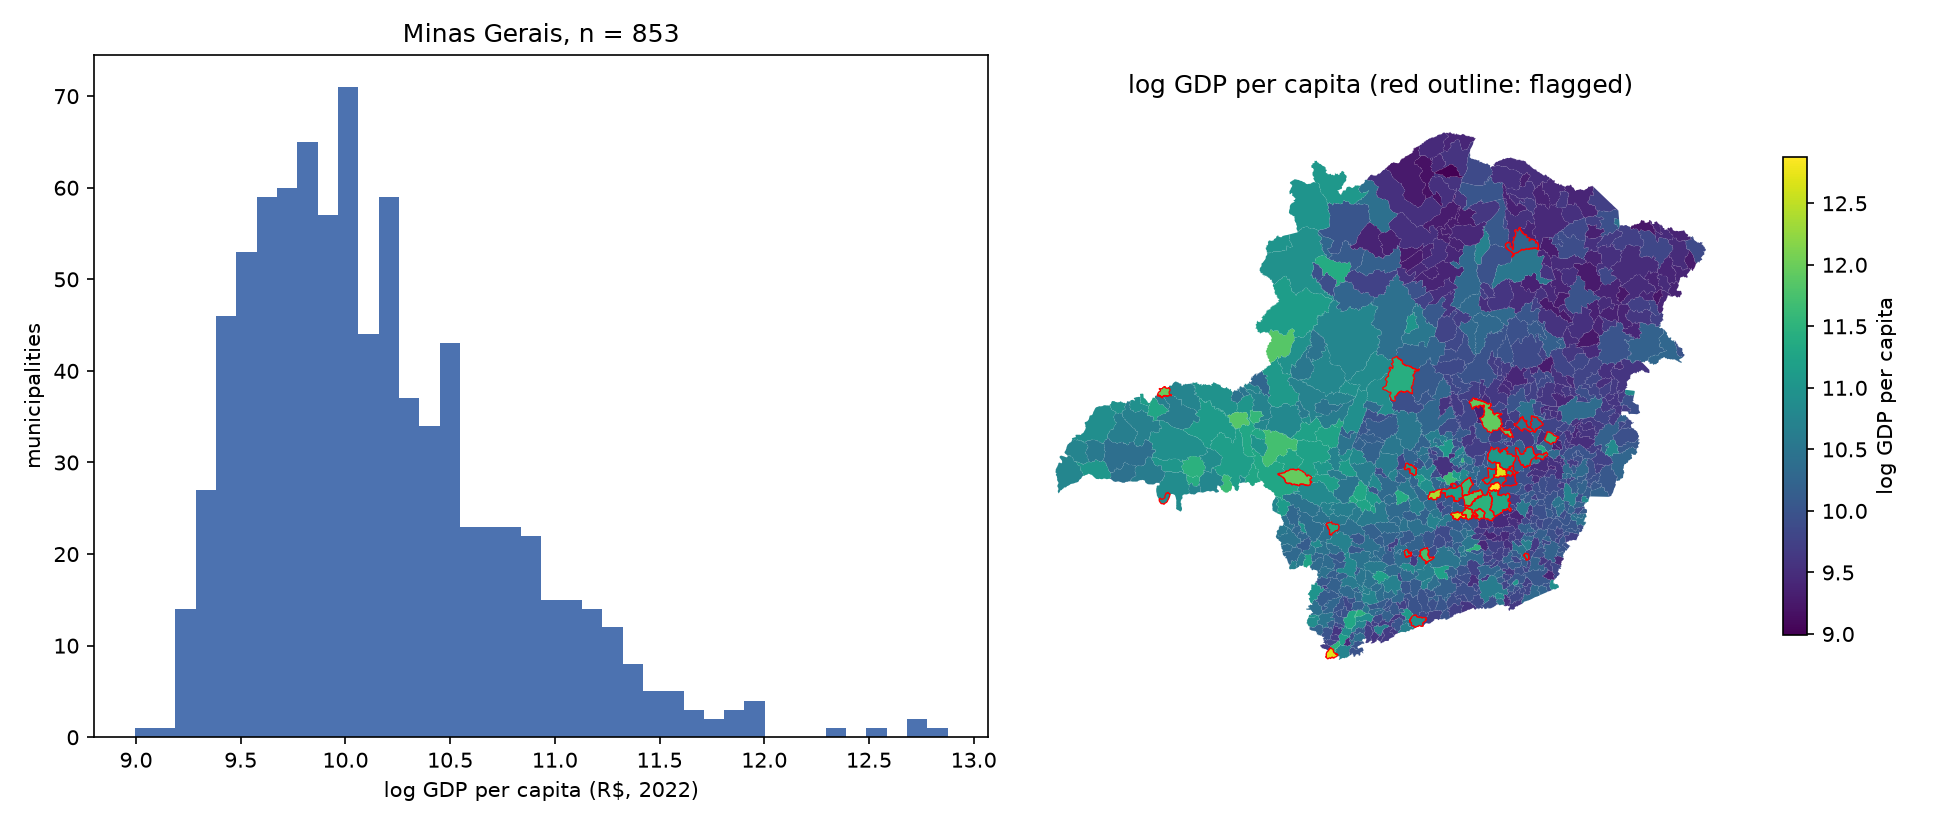
\includegraphics[width=0.92\linewidth]{labels_overview.png}
\caption{Official 2022 log GDP per capita of the 853 municipalities (IBGE). The south-west (Triângulo) and the
Belo Horizonte metro are rich; the north and north-east (Jequitinhonha, Norte de Minas) are poor.}
\label{fig:labels}
\end{figure}

\begin{table}[!htbp]
\centering\small
\caption{Data layers. All are free; all raster layers are averaged onto the same 1\,km grid (EPSG:31983).}
\label{tab:data}
\begin{tabularx}{\linewidth}{@{}l >{\raggedright\arraybackslash}p{6.8cm} L@{}}
\toprule
Layer & Source (year) & Role \\
\midrule
Satellite embeddings & Google GSED (Earth Engine, 2022), 64 bands, 10\,m & Main image input \\
Night lights & VIIRS DNB annual V2.2, \texttt{average\_masked} (2022) & Stage B proxy label; NTL benchmark \\
Land cover & ESA WorldCover v200 (2021) & Masking, fact sentences, caption checks, baseline V2 \\
POIs, roads, waterways & OpenStreetMap, Geofabrik extract of 1 Jan 2023 & POI counts (10 classes), road km (4 classes) \\
Buildings & Microsoft Global ML Building Footprints (10.0\,M) + OSM (0.36\,M) & Caption checks \\
Caption imagery & Esri World Imagery, zoom 17 ($\approx$1.1\,m/px), 768$\times$768\,px & VLM input only \\
GDP, value added & IBGE PIB dos Municípios (GDP 2022; sector shares 2021) & Stage C target; error analysis \\
Population & IBGE Census 2022 & GDP per capita \\
Boundaries, regions & IBGE Malha 2022; Regiões Geográficas Imediatas (2017) & Cell assignment; spatial blocks \\
\bottomrule
\end{tabularx}
\end{table}

\paragraph{Grid and cells.} The state is covered by a 1186\,$\times$\,963 grid of 1\,km cells in SIRGAS\,2000 / UTM
23S; 586{,}873 cells have their centre inside a municipality. GSED, VIIRS and WorldCover are read directly at 1\,km
from Earth Engine (GSED at 10\,m in the grid CRS, then averaged). We drop 1{,}441 cells that are $\geq$90\% water and
10{,}266 cells that are $\geq$95\% tree or bare ground \emph{and} have no built-up area, light, POI or road. The
remaining 575{,}166 cells carry the 64 GSED numbers, log night light $\log(1+\text{NTL})$, land-cover shares, POI
counts and road lengths (Table~\ref{tab:data}). Night lights are never used as a GDP proxy target: the target is
always official IBGE GDP.

%=====================================================================
\section{Method}

\begin{figure}[!htbp]
\centering
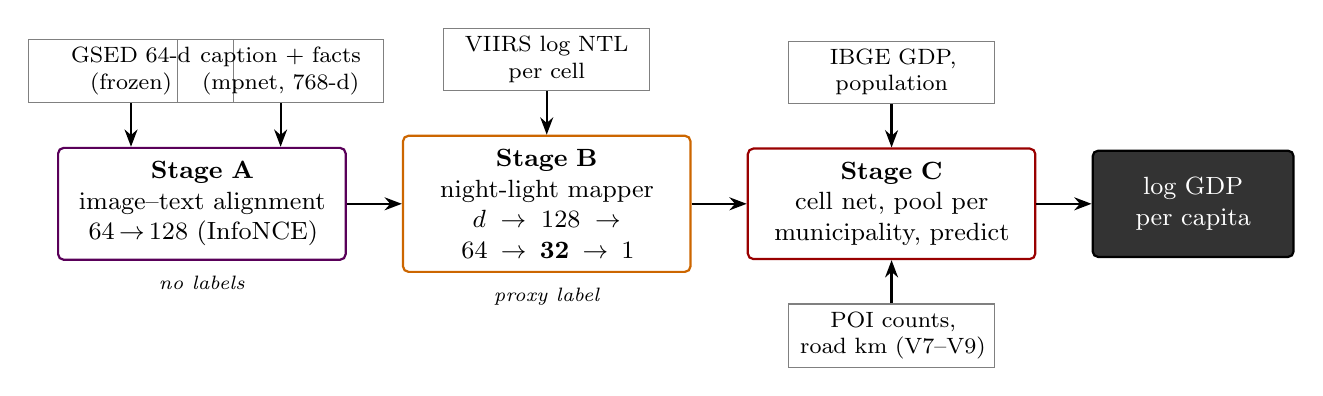
\begin{tikzpicture}[node distance=0.55cm and 0.7cm,
  box/.style={draw,thick,rounded corners=2pt,align=center,inner sep=5pt,font=\small,text width=3.3cm,minimum height=1.35cm},
  inp/.style={draw=gray,align=center,inner sep=3pt,font=\footnotesize,text width=2.4cm},
  arr/.style={-{Stealth[length=2.2mm]},thick}]
  \node[box,draw=violet!70!black] (A) {\textbf{Stage A}\\image--text alignment\\64\,$\to$\,128 (InfoNCE)};
  \node[box,draw=orange!80!black,right=of A] (B) {\textbf{Stage B}\\night-light mapper\\$d\to128\to64\to\mathbf{32}\to1$};
  \node[box,draw=red!60!black,right=of B] (C) {\textbf{Stage C}\\cell net, pool per\\municipality, predict};
  \node[box,fill=black!80,text=white,right=of C,text width=2.2cm] (Y) {log GDP\\per capita};
  \node[inp,above=of A,xshift=-0.9cm] (g) {GSED 64-d\\(frozen)};
  \node[inp,above=of A,xshift=1.0cm] (t) {caption + facts\\(mpnet, 768-d)};
  \node[inp,above=of B] (n) {VIIRS log NTL\\per cell};
  \node[inp,above=of C] (y) {IBGE GDP,\\population};
  \node[inp,below=of C] (p) {POI counts,\\road km (V7--V9)};
  \draw[arr] (g) -- (A.north -| g); \draw[arr] (t) -- (A.north -| t); \draw[arr] (n) -- (B);
  \draw[arr] (y) -- (C); \draw[arr] (p) -- (C);
  \draw[arr] (A) -- (B); \draw[arr] (B) -- (C); \draw[arr] (C) -- (Y);
  \node[font=\scriptsize\itshape,below=2pt of A] {no labels};
  \node[font=\scriptsize\itshape,below=2pt of B] {proxy label};
\end{tikzpicture}
\caption{Pipeline. Stage A needs text only in training; at prediction time each cell enters through its embedding
alone. Variants skip stages (Table~\ref{tab:variants}); all stages are retrained in every cross-validation round.}
\label{fig:pipeline}
\end{figure}

\subsection{Text: captions and fact sentences}
We sample 10{,}000 kept cells, 2{,}000 per fold, stratified by built-up tercile and night-light decile so that towns
are oversampled relative to pasture. For each we download an Esri World Imagery crop of the cell and caption it with
Qwen2.5-VL-7B-Instruct on Kaggle (2$\times$T4, fp16, temperature 0.2, at most 200 new tokens). A 200-tile pilot showed
accurate but long captions (median 142 words, 12\% cut off at the token limit), so the final prompt asks for
\emph{at most 5 short sentences, under 90 words, covering built-up area and buildings, roads, vegetation and
farmland, water, and industry or mining; only what is clearly visible; no place names; no summary sentence}.

Each cell also gets 2--4 \emph{fact sentences} written from its data, e.g.\ ``Mostly built-up: 74\% built-up, 24\%
trees. 3 schools and 1 public building are mapped. 2.6 km of medium roads and 14.2 km of minor roads.'' Night lights
are deliberately left out of the facts so that the effects of text (RQ2) and steering (RQ1) stay separable.

\paragraph{Cleaning.} Captions are split into 60{,}023 sentences. Pass 1 removes filler (``the overall scene
suggests\ldots''). Pass 2 checks claims against the cell's data with a keyword lexicon: water words need water cover
or a mapped waterway; building words need built-up cover, buildings or POIs; industry or mining words need an
industry POI or enough built-up area; farm, forest, road and urban words have similar checks. Sentences with a
negation (``no river is visible'') skip the check. Pass 3 scores each tile against its cleaned caption with
RemoteCLIP ViT-B/32 and drops captions below the 5th percentile of a seeded 200-caption subset (246 captions). In total
84\% of sentences are kept; the removals are filler (4{,}183), industry (1{,}130), building (1{,}108), water
(1{,}046), road (1{,}039), farm (732), urban (66) and forest (35). Three text versions feed the ablations:
\texttt{full} (cleaned caption + facts), \texttt{raw} (uncleaned caption) and \texttt{facts} (no VLM at all).

\subsection{Stage A: image--text alignment}
GSED vectors are standardised with training-cell statistics. A two-layer projector maps the 64 GSED numbers to a
128-d unit vector ($64\to256\to128$, GELU, dropout 0.1); a second projector maps the frozen 768-d
\texttt{all-mpnet-base-v2} sentence embedding of the text to the same space. A symmetric InfoNCE loss with learnable
temperature (initial 0.07) pulls each cell towards its own text. We train on the $\approx$6{,}000 captioned cells of
the training municipalities (AdamW, lr $10^{-3}$, batch 256, early stopping on the validation fold's captions) and
then embed \emph{every} kept cell with the image projector. GSED is frozen, so Stage A can only reorganise the
information GSED already holds; it cannot add new information.

\subsection{Stage B: night-light steering}
A network $d\to128\to64\to32\to1$ (ReLU) predicts each cell's standardised $\log(1+\text{NTL})$ from its embedding
(raw GSED, $d=64$, or a Stage A embedding, $d=128$), trained on all training-fold cells and early-stopped on the
validation fold. The 32-number last hidden layer \textbf{z} is the steered embedding. The embedding paper does not
publish its layer widths; ours follow its three-hidden-layer shape.

\subsection{Stage C: from cells to municipalities}
Each cell's input (z, a Stage A embedding or raw GSED, plus optionally $\log(1+x)$ POI counts and road km) passes a
per-cell network (hidden 32 or 64, dropout 0.1, softplus output of 16 numbers). Outputs are pooled per municipality
(log-sum or mean), a municipal network $16\to16\to1$ predicts log total GDP, and log population is subtracted. Training
is full-batch on log GDP per capita (Adam, lr $10^{-3}$ halved after 50 epochs without improvement, early stopping on
a 100-epoch rolling mean of validation MSE, at most 3{,}000 epochs). The output bias starts at the training mean,
without which Adam could not reach the target scale in time. A 12-setting grid (hidden $\{32,64\}$ $\times$ weight
decay $\{10^{-4},10^{-3},10^{-2}\}$ $\times$ pooling \{log-sum, mean\}) is tuned on the validation fold, and the chosen
setting is retrained with 5 seeds whose mean is the prediction. Log-sum pooling won in 33 of 35 variant--rounds.
Finally a linear recalibration (official on predicted) is fitted on the validation fold and applied to test.

\subsection{Baselines, hybrid and variants}
V1 is the night-light benchmark of Hu and Yao (2022) and the embedding paper: OLS of log GDP per capita on
$\log(1+\sum\text{NTL})-\log(\text{pop})$, linear or quadratic chosen on validation. V2 is a ridge on mean land-cover
shares, log cell count and log population. V11 is a ridge on mean embeddings (each embedding type separately) and V12
LightGBM on the same municipal features. V10 blends the best of V3--V9 (by validation RMSE) with V1:
$\alpha\,\hat y_{\text{model}}+(1-\alpha)\,\hat y_{\text{V1}}$, $\alpha\in\{0,0.25,\ldots,1\}$ chosen on validation.

\begin{table}[!htbp]
\centering\small
\caption{Model variants. All use the same five rounds; A = Stage A, B = Stage B, C = Stage C.}
\label{tab:variants}
\begin{tabularx}{\linewidth}{@{}l l L@{}}
\toprule
ID & Pipeline & Question \\
\midrule
V1 & night lights only (OLS) & benchmark \\
V2 & land-cover shares $\to$ ridge & is a simple model enough? \\
V3 & raw GSED $\to$ C & base value of embeddings \\
V4 & raw GSED $\to$ B $\to$ C & RQ1: steering (reproduces the embedding paper) \\
V5 & A(full) $\to$ C & text without steering \\
V6 & A(full) $\to$ B $\to$ C & RQ2: text + steering \\
V7 & A(full) $\to$ B $\to$ C + POI/roads & RQ3: full model \\
V8 & as V7, uncleaned captions & value of cleaning \\
V9 & as V7, fact sentences only & is the VLM needed? \\
V10 & best of V3--V9 blended with V1 & RQ4: hybrid \\
V11 & ridge on mean embeddings & simple check of each embedding \\
V12 & LightGBM on municipal features & strong off-the-shelf baseline \\
\bottomrule
\end{tabularx}
\end{table}

\subsection{Evaluation}
The 70 IBGE immediate regions are the spatial blocks. Of 10{,}000 random assignments of regions to 5 folds we keep
the one most balanced in municipality count, mean and spread of log GDP per capita and urban share
(Figure~\ref{fig:folds}; 160--184 municipalities and 14 regions per fold). In round $r$, fold $r$ is the test fold,
fold $r{+}1$ validates, and the other three train. Test municipalities never influence any stage, scaler, threshold,
hyperparameter, hybrid weight or caption used in training; captions of test cells are never loaded. We pool the 853
test predictions and report \R, RMSE and MAE. For each research question we compute the RMSE difference with a 95\%
block bootstrap that resamples the 70 regions 2{,}000 times; an interval containing 0 is reported as ``no clear effect''.

\begin{figure}[!htbp]
\centering
\begin{subfigure}[b]{0.46\linewidth}\centering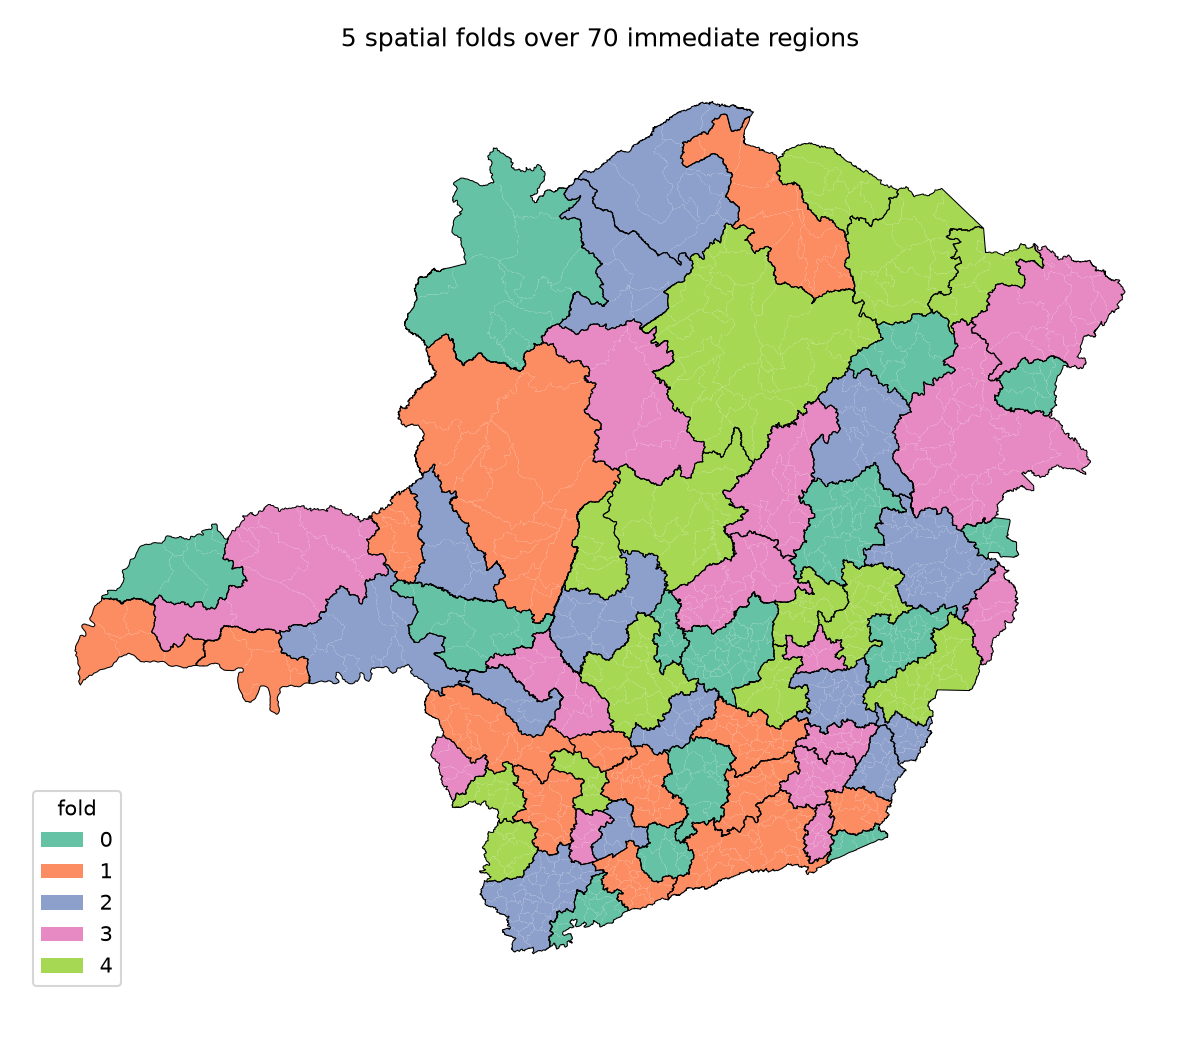
\includegraphics[width=\linewidth]{folds_map.png}
\caption{Five spatial folds over the 70 immediate regions.}\label{fig:folds}\end{subfigure}\hfill
\begin{subfigure}[b]{0.5\linewidth}\centering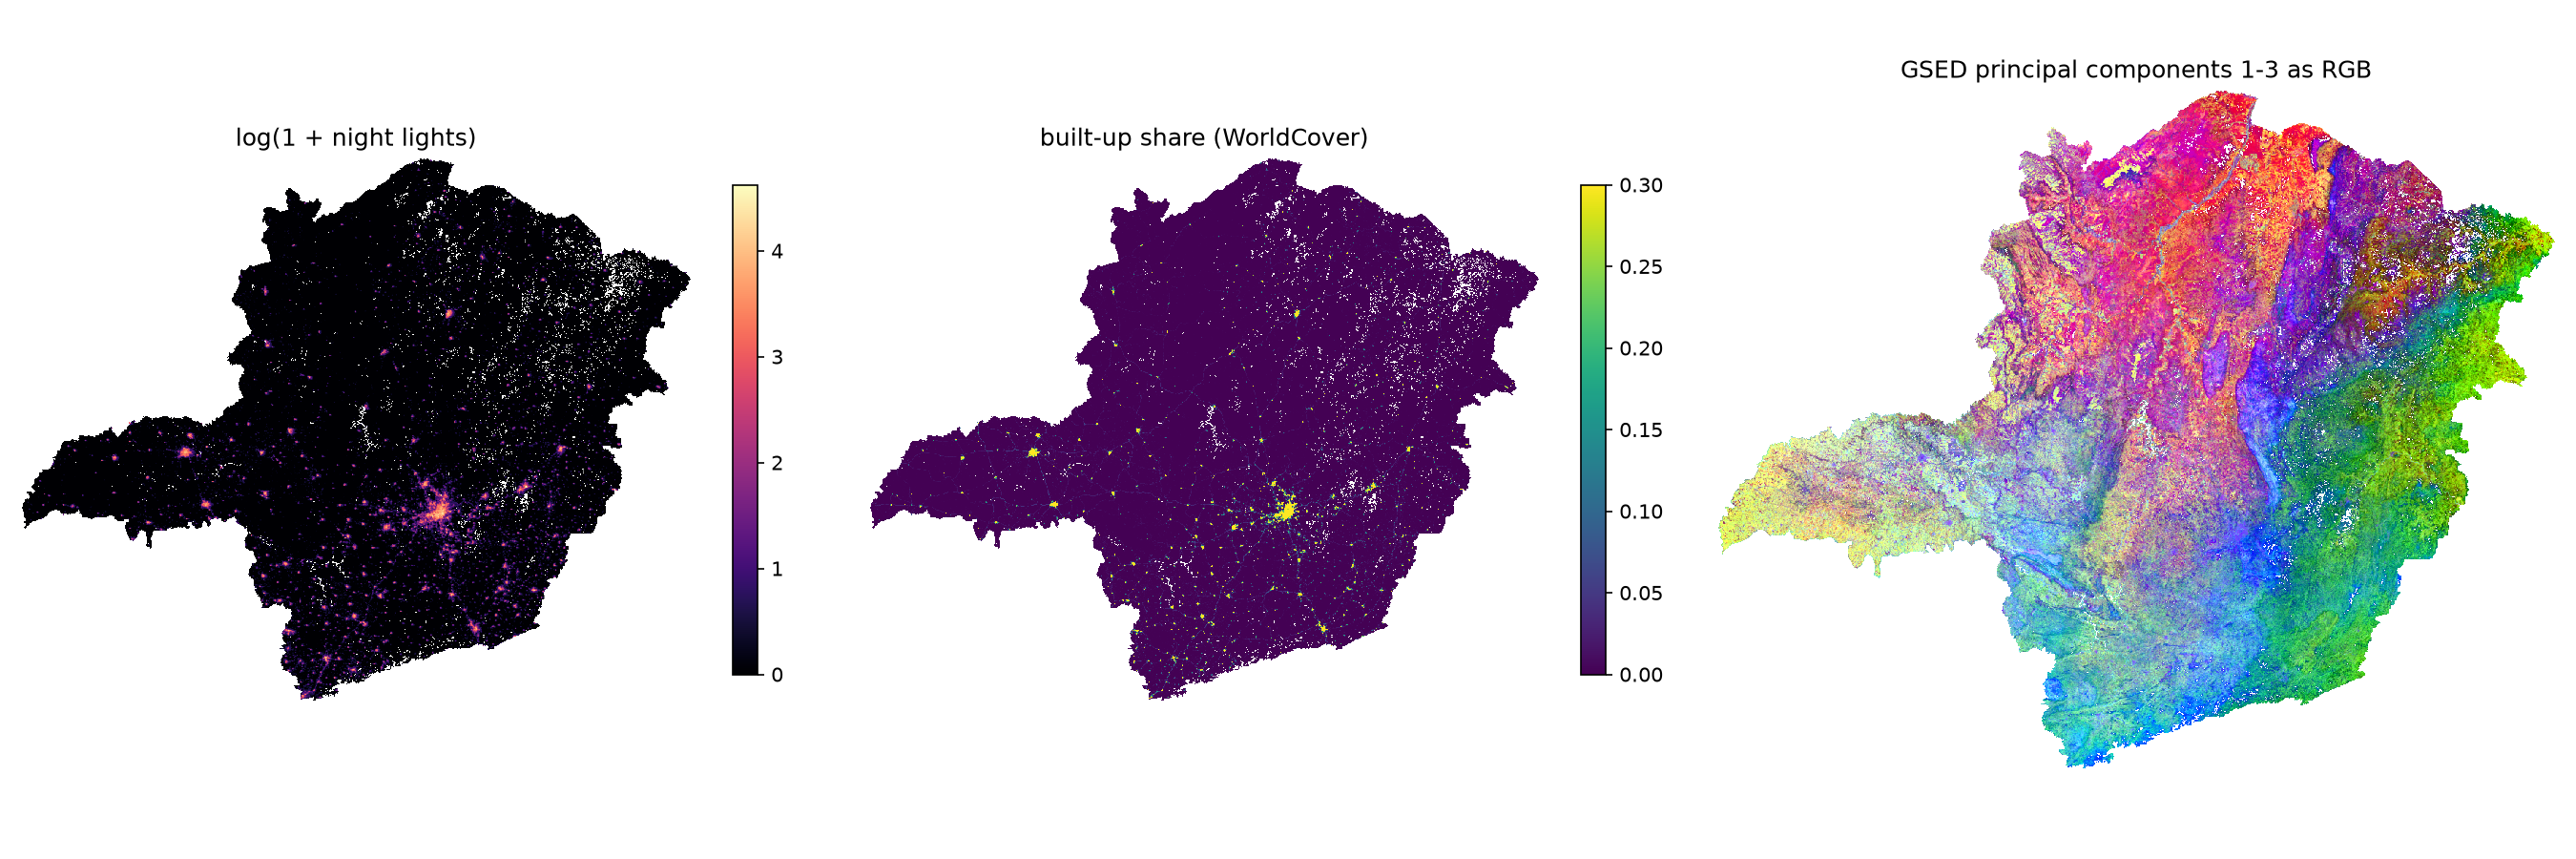
\includegraphics[width=\linewidth]{cells_qc.png}
\caption{Quality check: log night light, built-up share, GSED principal components as RGB.}\end{subfigure}
\caption{Spatial cross-validation design and the cell table.}
\end{figure}

%=====================================================================
\section{Results}

\subsection{Main results}

\begin{table}[!htbp]
\centering\small
\caption{Out-of-sample results, all 853 municipalities pooled over 5 rounds (log GDP per capita). ``Unflagged''
excludes the 34 municipalities flagged for industry share above 60\% or top-1\% GDP per capita. Calibration
slope: regression of official on predicted (1 = no bias).}
\label{tab:results}
\begin{tabular}{@{}llrrrrrr@{}}
\toprule
 & & \R & RMSE & MAE & RMSE sd & RMSE & calib. \\
ID & Model & & & & (rounds) & unflagged & slope \\
\midrule
V1 & night lights only & 0.271 & 0.510 & 0.406 & 0.015 & 0.477 & 0.97 \\
V2 & land cover $\to$ ridge & 0.124 & 0.559 & 0.373 & 0.155 & 0.508 & 0.60 \\
V3 & GSED $\to$ C & 0.459 & 0.439 & 0.323 & 0.020 & 0.408 & 0.91 \\
V4 & GSED $\to$ B $\to$ C & 0.441 & 0.446 & 0.333 & 0.054 & 0.406 & 0.84 \\
V5 & A(full) $\to$ C & 0.483 & 0.429 & 0.313 & 0.021 & 0.391 & 0.90 \\
V6 & A(full) $\to$ B $\to$ C & 0.501 & 0.422 & 0.308 & 0.019 & 0.378 & 0.94 \\
V7 & V6 + POI/roads & 0.502 & 0.421 & 0.306 & 0.029 & 0.373 & 0.96 \\
V8 & V7, uncleaned captions & 0.501 & 0.422 & 0.309 & 0.048 & 0.380 & 0.93 \\
V9 & V7, facts only & 0.483 & 0.429 & 0.318 & 0.049 & 0.385 & 0.92 \\
\textbf{V10} & \textbf{hybrid (best + V1)} & \textbf{0.523} & \textbf{0.412} & \textbf{0.302} & 0.035 & 0.381 & 0.95 \\
V11 & ridge, mean A(full) emb. & 0.397 & 0.463 & 0.330 & 0.038 & 0.395 & 0.90 \\
V11 & ridge, mean raw GSED & 0.345 & 0.483 & 0.346 & 0.064 & 0.416 & 0.90 \\
V12 & LightGBM & 0.386 & 0.468 & 0.335 & 0.047 & 0.401 & 0.96 \\
\bottomrule
\end{tabular}
\end{table}

Table~\ref{tab:results} gives the main results. Every Stage C model (V3--V10) beats the night-light benchmark by a
wide margin (\R{} 0.44--0.52 vs.\ 0.27), and also beats ridge and LightGBM on the same embeddings (0.35--0.40). The
deep pooling therefore earns its place: learning which cells matter, rather than averaging them, is worth about 0.1
in \R. The best model is the hybrid V10 (\R{} 0.523, RMSE 0.412); without the 34 flagged municipalities its RMSE
drops to 0.381. Figure~\ref{fig:scatter} shows its predictions against official values next to V1's: V1 squeezes
almost all municipalities into a narrow band, while V10 spreads along the diagonal but still pulls the extremes
towards the middle. Other ensemble variants are reported in the repository (\texttt{reports/tables/main\_results.csv}).

\begin{figure}[!htbp]
\centering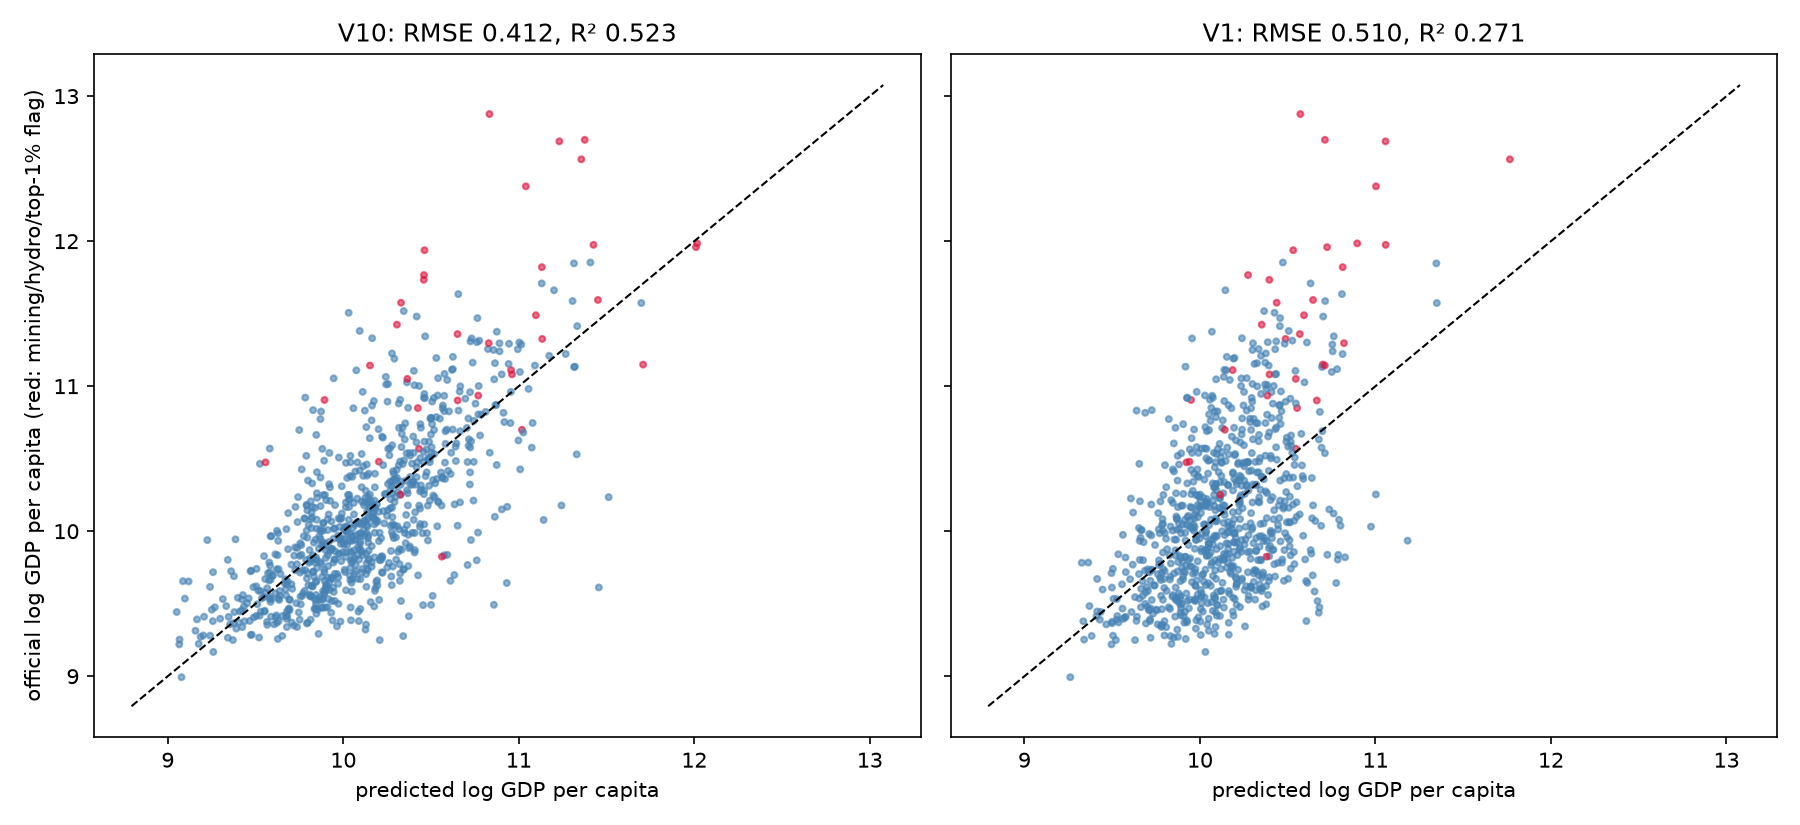
\includegraphics[width=\linewidth]{pred_vs_official.png}
\caption{Predicted vs.\ official log GDP per capita, test predictions of all five rounds. Left: hybrid V10; right:
night lights only (V1). Red: flagged mining, hydro or top-1\% municipalities.}
\label{fig:scatter}
\end{figure}

\begin{table}[!htbp]
\centering\small
\caption{Research-question tests: RMSE difference (first minus second model) with 95\% block-bootstrap interval over
the 70 regions. Negative = first model better.}
\label{tab:rq}
\begin{tabular}{@{}llrl@{}}
\toprule
Question & Comparison & $\Delta$RMSE [95\% CI] & Verdict \\
\midrule
RQ1 night-light steering & V4 vs V3 & $+0.007$ [$-0.028$, $+0.041$] & no clear effect \\
RQ2 text + steering & V6 vs V4 & $-0.025$ [$-0.050$, $+0.004$] & no clear effect (borderline) \\
RQ3 POIs and roads on top & V7 vs V6 & $-0.001$ [$-0.017$, $+0.016$] & no clear effect \\
RQ4 hybrid vs best single & V10 vs V8 & $-0.010$ [$-0.035$, $+0.015$] & no clear effect \\
\bottomrule
\end{tabular}
\end{table}

\subsection{Research questions 1--4}
\textbf{RQ1, steering.} Steering raw GSED with night lights does not help: V4 is slightly worse than V3 and the
interval is centred on zero. This does \emph{not} reproduce the embedding paper's gain. Stage B itself works
(validation \R{} 0.74--0.85 for log night light; Table~\ref{tab:diag}), so the steered space does encode light, but
the 32-number bottleneck discards information that Stage C could otherwise use, and light is already partly
recoverable from GSED.

\textbf{RQ2, text.} Aligning with text is the largest single gain: V6 improves on V4 by 0.025 RMSE (about 2.5\% in
GDP per capita), and V5 improves on V3 by 0.010 without steering. The interval only just includes zero. The ablations
point the same way: uncleaned captions (V8) and fact sentences alone (V9) are no better than the cleaned
captions plus facts (V7), so the gain does not hinge on the vision--language model or on cleaning.

\textbf{RQ3, POIs and roads.} Adding POI counts and road lengths as numbers changes nothing (V7 vs V6). The fact
sentences already mention POIs and roads, so their information reaches the model through text; OSM is also sparse in
rural Minas, and the OSM-completeness term has no effect on errors (Section~\ref{sec:errors}).

\textbf{RQ4, hybrid.} The hybrid is the best model overall, but its edge over the best single model chosen on
validation (V8) is small and not significant. In three rounds the validation-optimal weight was $\alpha=1$ (no night
lights), in two $\alpha=0.75$; the base model also differs by round (V6, V5, V8, V3, V3). Much of V10's advantage is
thus picking the best Stage C model per round on validation rather than blending.

\paragraph{A lesson on honest re-testing.} The first complete run (before Stage C was revised) gave a different
picture: V3 RMSE 0.555, V4 0.491, and RQ1 ``V4 better'' with an interval excluding zero ($-0.064$ [$-0.115$,
$-0.019$]). Inspecting \emph{validation} curves showed that Stage C predictions were over-dispersed and that plain sum
pooling never won. Adding the validation recalibration and mean pooling, and replacing sum pooling in the grid, cut V3's
RMSE by 21\% and V4's by 9\%, and the apparent steering effect vanished: steering had been compensating for a
poorly calibrated aggregator. All changes were chosen on validation data only, but we made them after seeing the
first test results, which we report here as a researcher degree of freedom.

\subsection{Did each stage do its job?}

\begin{table}[!htbp]
\centering\small
\caption{Stage diagnostics, mean over 5 rounds (validation fold). Stage A: image$\to$text recall@k within groups of
256 validation pairs (chance recall@10 $\approx$ 4\%) and a linear probe from the embedding to built-up share. Stage B:
validation \R{} and RMSE of standardised log night light; 81\% of training cells are unlit.}
\label{tab:diag}
\begin{tabular}{@{}lrrrr@{\hspace{1.5em}}lrr@{}}
\toprule
\multicolumn{5}{c}{Stage A} & \multicolumn{3}{c}{Stage B} \\
\cmidrule(r{1.2em}){1-5}\cmidrule{6-8}
Text & R@1 & R@5 & R@10 & probe \R & Input & \R & RMSE \\
\midrule
full (cleaned + facts) & 0.123 & 0.361 & 0.522 & 0.67 & raw GSED & 0.775 & 0.176 \\
raw caption & 0.065 & 0.229 & 0.349 & 0.68 & A(full) & 0.763 & 0.181 \\
facts only & 0.122 & 0.376 & 0.551 & 0.64 & A(raw) & 0.761 & 0.182 \\
 & & & & & A(facts) & 0.752 & 0.185 \\
\bottomrule
\end{tabular}
\end{table}

Stage A aligns image and text far above chance: the right text ranks among the top 10 of 256 candidates for
52\% of validation cells with the full text, against about 4\% by chance (Table~\ref{tab:diag}). Raw captions align
worst (35\%) and fact sentences best (55\%), which is expected: the facts are computed from land cover, roads and POIs,
which GSED can see, while the free-form captions also contain sentences GSED cannot match. The embedding keeps basic
land information (probe \R{} 0.64--0.68 for built-up share). Stage B predicts night light well from any embedding,
best from raw GSED, consistent with Stage A only reshaping GSED.

\begin{figure}[!htbp]
\centering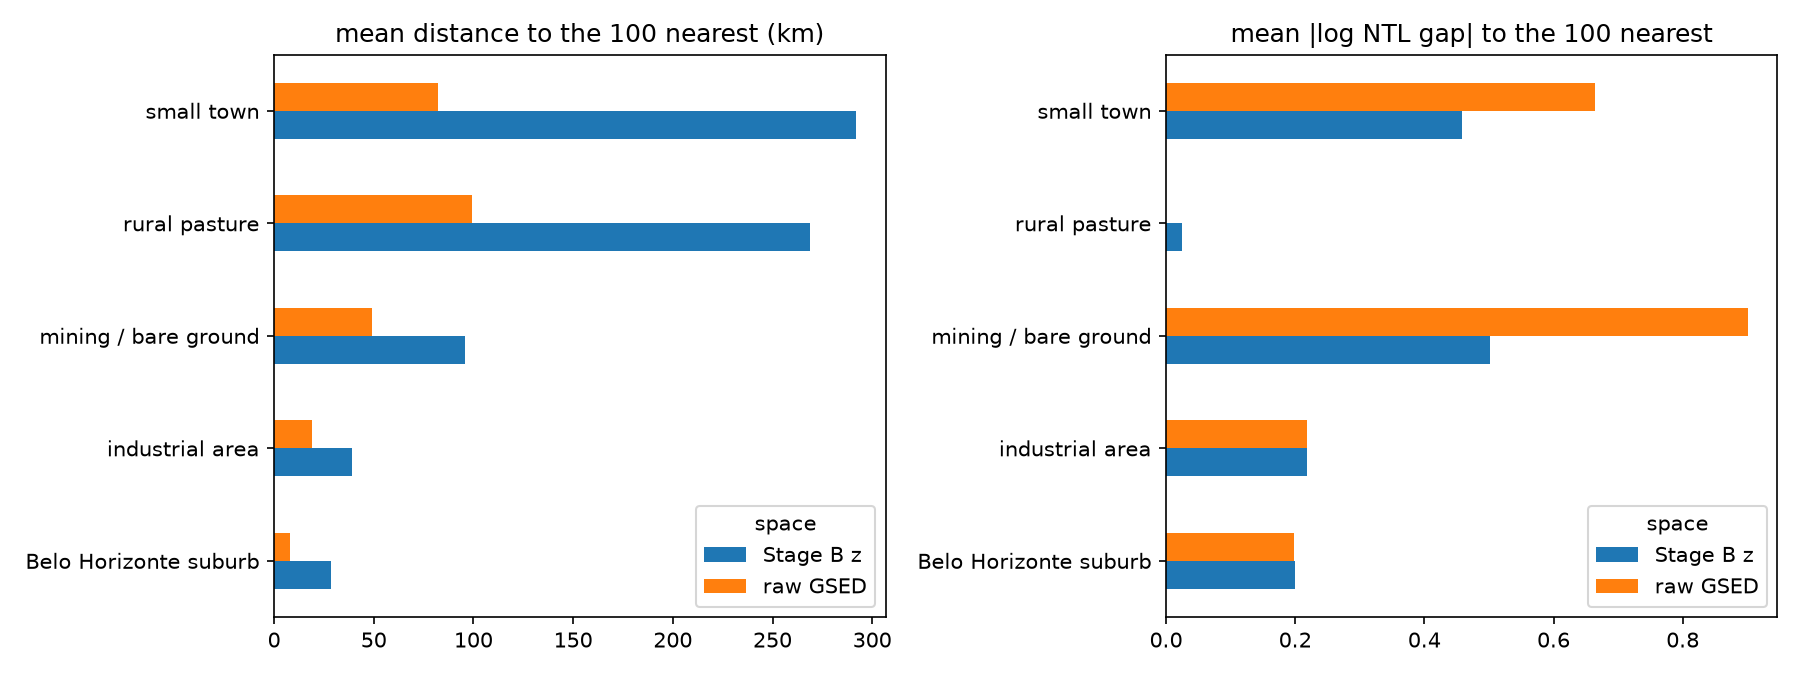
\includegraphics[width=0.92\linewidth]{neighbours_raw_vs_z.png}
\caption{The embedding paper's neighbour check, round 0. For five reference cells, the 100 nearest cells by cosine
similarity in raw GSED and in the steered space z: mean geographic distance (left) and mean absolute gap in log night
light (right).}
\label{fig:neigh}
\end{figure}

Figure~\ref{fig:neigh} repeats the embedding paper's neighbour check. In the steered space z, a cell's nearest
neighbours are 2--4 times farther away (e.g.\ 82 vs 292\,km for a small town) but more alike in night light for the
small town (log-NTL gap 0.66 $\to$ 0.46) and the mining cell (0.90 $\to$ 0.50), and equal for the industrial and Belo
Horizonte cells. Steering does what the paper describes, turning ``looks like its neighbours'' into ``is as active
as'', yet this did not translate into better municipal GDP here (RQ1).

%=====================================================================
\section{Where and why the model fails (RQ5)}
\label{sec:errors}

\begin{figure}[!htbp]
\centering
\begin{subfigure}[b]{0.32\linewidth}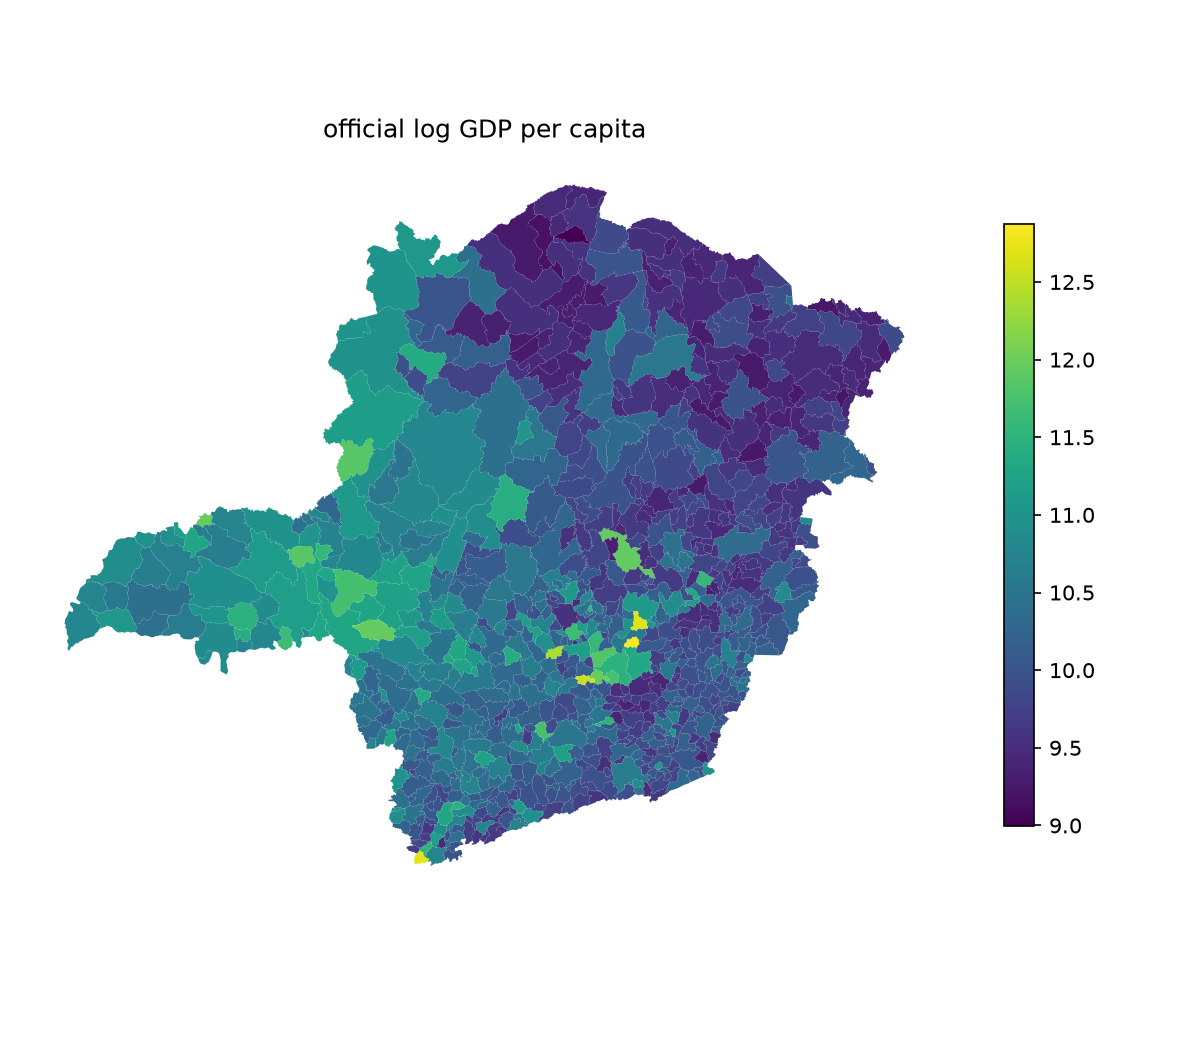
\includegraphics[width=\linewidth]{map_official.png}\caption{Official}\end{subfigure}\hfill
\begin{subfigure}[b]{0.32\linewidth}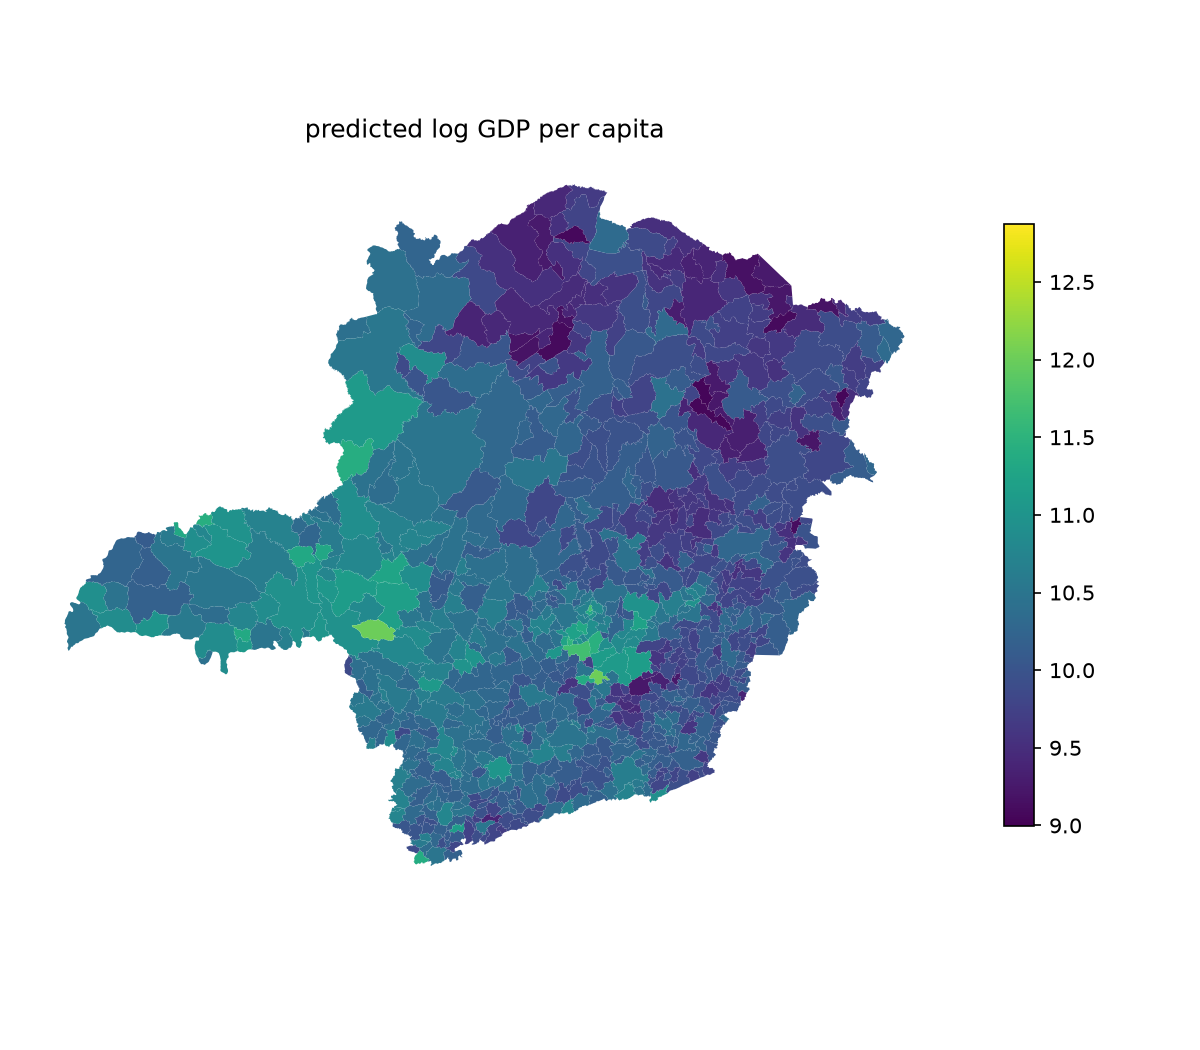
\includegraphics[width=\linewidth]{map_predicted.png}\caption{Predicted (V10)}\end{subfigure}\hfill
\begin{subfigure}[b]{0.32\linewidth}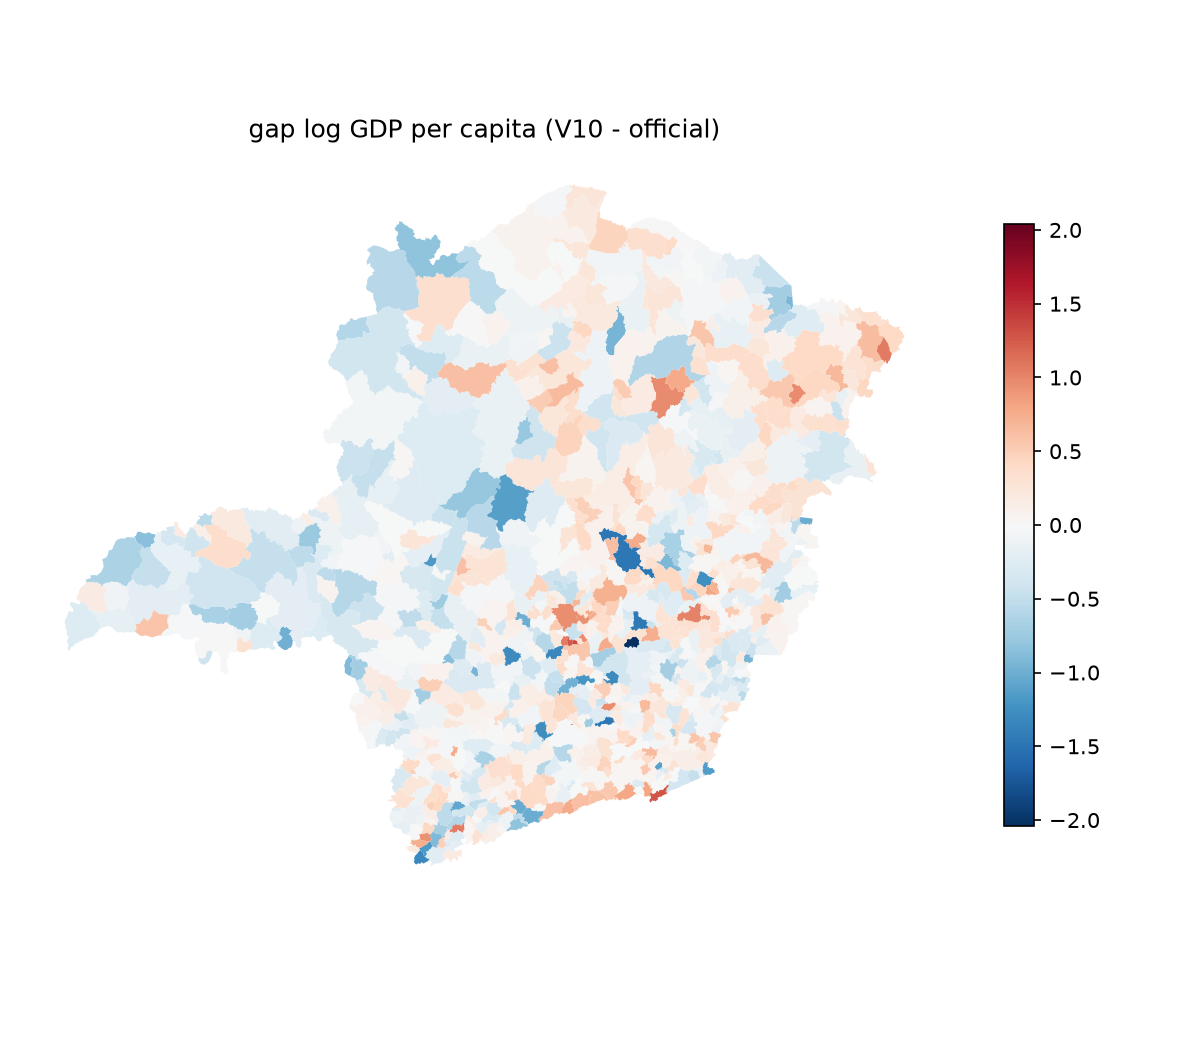
\includegraphics[width=\linewidth]{map_gap.png}\caption{Gap (V10 $-$ official)}\end{subfigure}
\caption{Municipal maps of log GDP per capita, same colour scale for official and predicted. Blue: under-predicted;
red: over-predicted.}
\label{fig:maps}
\end{figure}

The predicted map reproduces the main geography (Figure~\ref{fig:maps}): the rich Triângulo and south, the Belo
Horizonte metro, and the poor north-east. The gaps are spatially clustered: Moran's I of the test residuals over
neighbouring municipalities is 0.16 for V10 ($p=0.001$), half the 0.33 of night lights alone. The embedding model
removes much of the regional bias of night lights, but a regional factor remains.

\begin{table}[!htbp]
\centering\small
\caption{Absolute error of V10 and V1 regressed on municipality traits (OLS, standard errors clustered by immediate
region, $n=853$). Sector shares are from 2021.}
\label{tab:errreg}
\begin{tabular}{@{}lrrrr@{}}
\toprule
 & \multicolumn{2}{c}{V10 hybrid} & \multicolumn{2}{c}{V1 night lights} \\
Term & coef. (SE) & $p$ & coef. (SE) & $p$ \\
\midrule
official log GDP per capita & 0.081 (0.035) & 0.02 & 0.190 (0.037) & $<$0.001 \\
built-up share & 0.836 (0.473) & 0.08 & 0.791 (0.250) & 0.002 \\
services share of value added & $-0.285$ (0.132) & 0.03 & $-0.332$ (0.123) & 0.007 \\
industry share of value added & 0.185 (0.121) & 0.13 & $-0.107$ (0.102) & 0.29 \\
flagged (mining/hydro/top 1\%) & 0.165 (0.090) & 0.07 & 0.272 (0.079) & $<$0.001 \\
OSM completeness & $-0.018$ (0.082) & 0.82 & $-0.099$ (0.054) & 0.07 \\
\bottomrule
\end{tabular}
\end{table}

\paragraph{Errors grow with income, less than for night lights.} Table~\ref{tab:errreg} mirrors the embedding paper's
error regression. IBGE publishes no per-municipality data-quality score, so we analyse income and economic structure
instead. For both models the absolute error rises with official income, but the slope for V10 is less than half that
of V1 (0.08 vs 0.19 per log point), and the LOWESS curves in Figure~\ref{fig:errinc} show the same. Errors are smaller
where services dominate the economy and larger in flagged municipalities, though for V10 the flag is only weakly
significant. OSM completeness does not matter for either model.

\begin{figure}[!htbp]
\centering
\begin{subfigure}[b]{0.48\linewidth}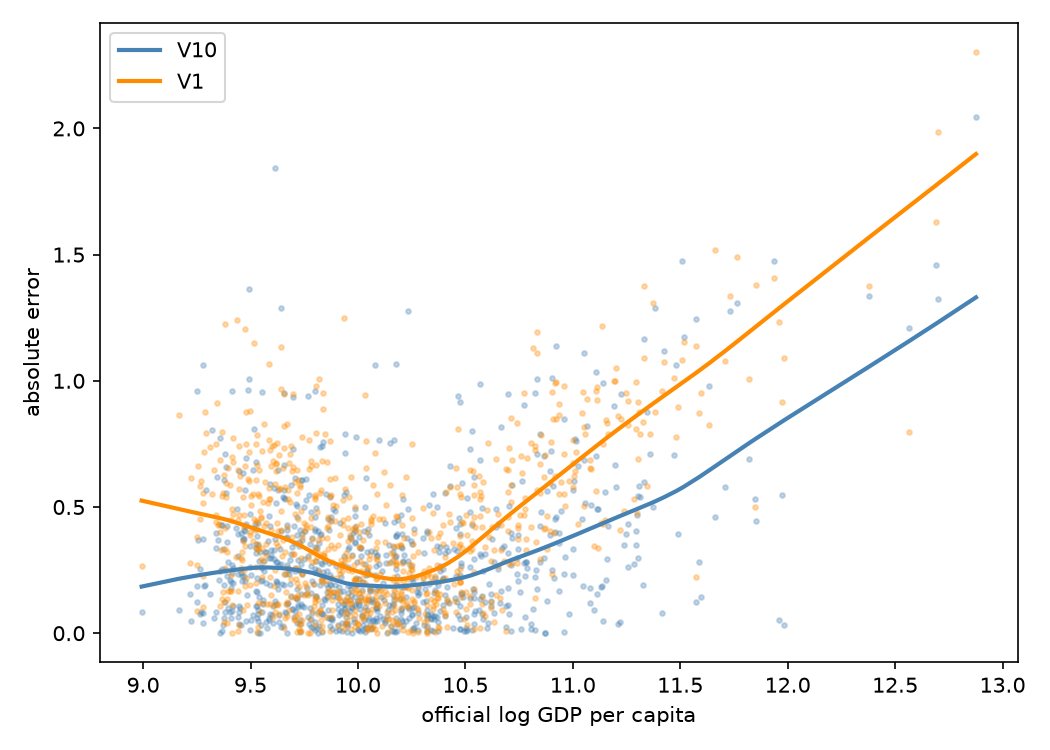
\includegraphics[width=\linewidth]{error_vs_income.png}
\caption{Absolute error vs.\ official income, LOWESS.}\label{fig:errinc}\end{subfigure}\hfill
\begin{subfigure}[b]{0.48\linewidth}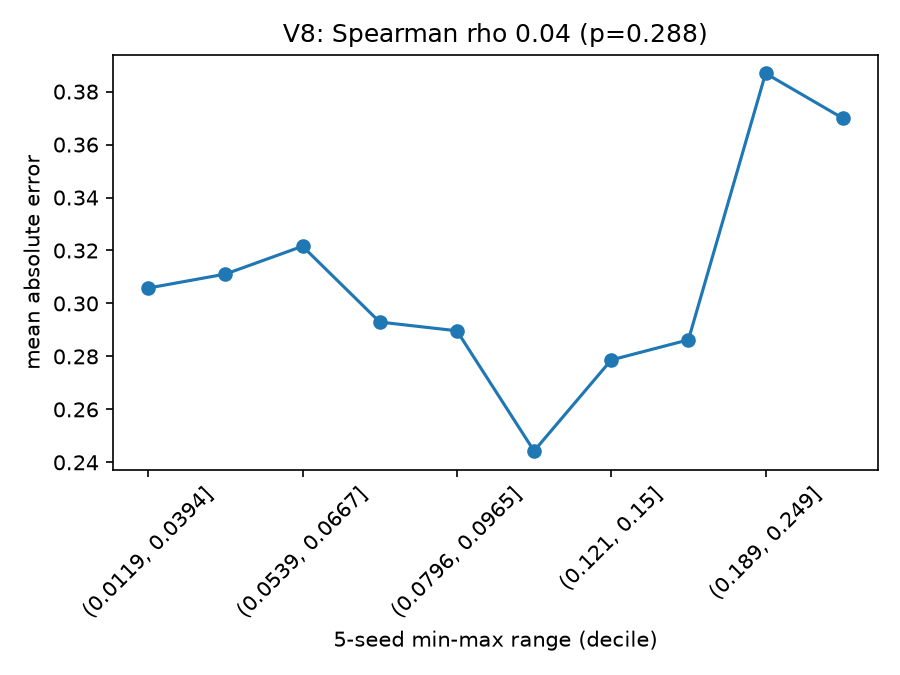
\includegraphics[width=\linewidth]{uncertainty_vs_error.png}
\caption{Ensemble spread vs.\ error (V8, 5 seeds).}\label{fig:unc}\end{subfigure}
\caption{Error structure and uncertainty.}
\end{figure}

\paragraph{The ten largest gaps.} Seven of the ten largest errors are under-predictions of mining or heavy-industry
municipalities (Table~\ref{tab:top10}). Catas Altas, Conceição do Mato Dentro, São Gonçalo do Rio Abaixo and Itatiaiuçu
host large iron-ore mines, Ouro Branco a large steel mill, and Extrema a logistics and industrial hub on the
São Paulo highway. In each, a handful of cells produce most of the output, while the sampled tiles show forest,
pasture and rock, and their captions say ``no industrial activity is visible''. Satellites cannot see a mine's
revenue, as the proposal anticipated. The three over-predictions are small towns with large public-sector shares
(39--48\%): Santa Cruz de Minas, one of Brazil's smallest municipalities and almost entirely urban next to São João
del-Rei, and Mário Campos, a Belo Horizonte commuter town, look as built-up as richer places but residents earn
elsewhere. These reasons are candidates from sector shares and public knowledge, not proof.

\begin{table}[!htbp]
\centering\small
\caption{The ten largest gaps of V10 (predicted minus official log GDP per capita) and candidate reasons.}
\label{tab:top10}
\begin{tabular}{@{}lrrrl@{}}
\toprule
Municipality & official & gap & industry & candidate reason \\
\midrule
Catas Altas & 12.88 & $-2.04$ & 81\% & iron-ore mining \\
Santa Cruz de Minas & 9.61 & $+1.84$ & 8\% & tiny urban commuter town, public sector 42\% \\
Ressaquinha & 11.51 & $-1.48$ & 50\% & single large plant (not identified) \\
Conceição do Mato Dentro & 11.94 & $-1.48$ & 80\% & iron-ore mine and pipeline \\
São Gonçalo do Rio Abaixo & 12.69 & $-1.46$ & 78\% & iron-ore mine \\
Mário Campos & 9.49 & $+1.37$ & 8\% & Belo Horizonte commuter town \\
Itatiaiuçu & 12.38 & $-1.34$ & 80\% & iron-ore mining \\
Extrema & 12.70 & $-1.32$ & 26\% & logistics and industry hub \\
Ouro Branco & 11.77 & $-1.31$ & 72\% & integrated steel mill \\
Chiador & 9.64 & $+1.29$ & 3\% & small public-sector economy (48\%) \\
\bottomrule
\end{tabular}
\end{table}

\paragraph{Uncertainty.} The spread of the 5-seed ensemble does not track the error (Spearman $\rho=0.04$, $p=0.29$;
Figure~\ref{fig:unc}). Seed variation measures optimisation noise, not the systematic error of a mining town, so it
should not be used as a confidence interval.

\paragraph{A 1\,km activity map.} Because every municipality is tested exactly once, we can assemble an out-of-sample
map of Stage B's predicted night light for every cell, each taken from the round in which its municipality was in
the test fold (Figure~\ref{fig:activity}). It is a relative activity index for display, not a GDP map.

\begin{figure}[!htbp]
\centering
\begin{subfigure}[b]{0.5\linewidth}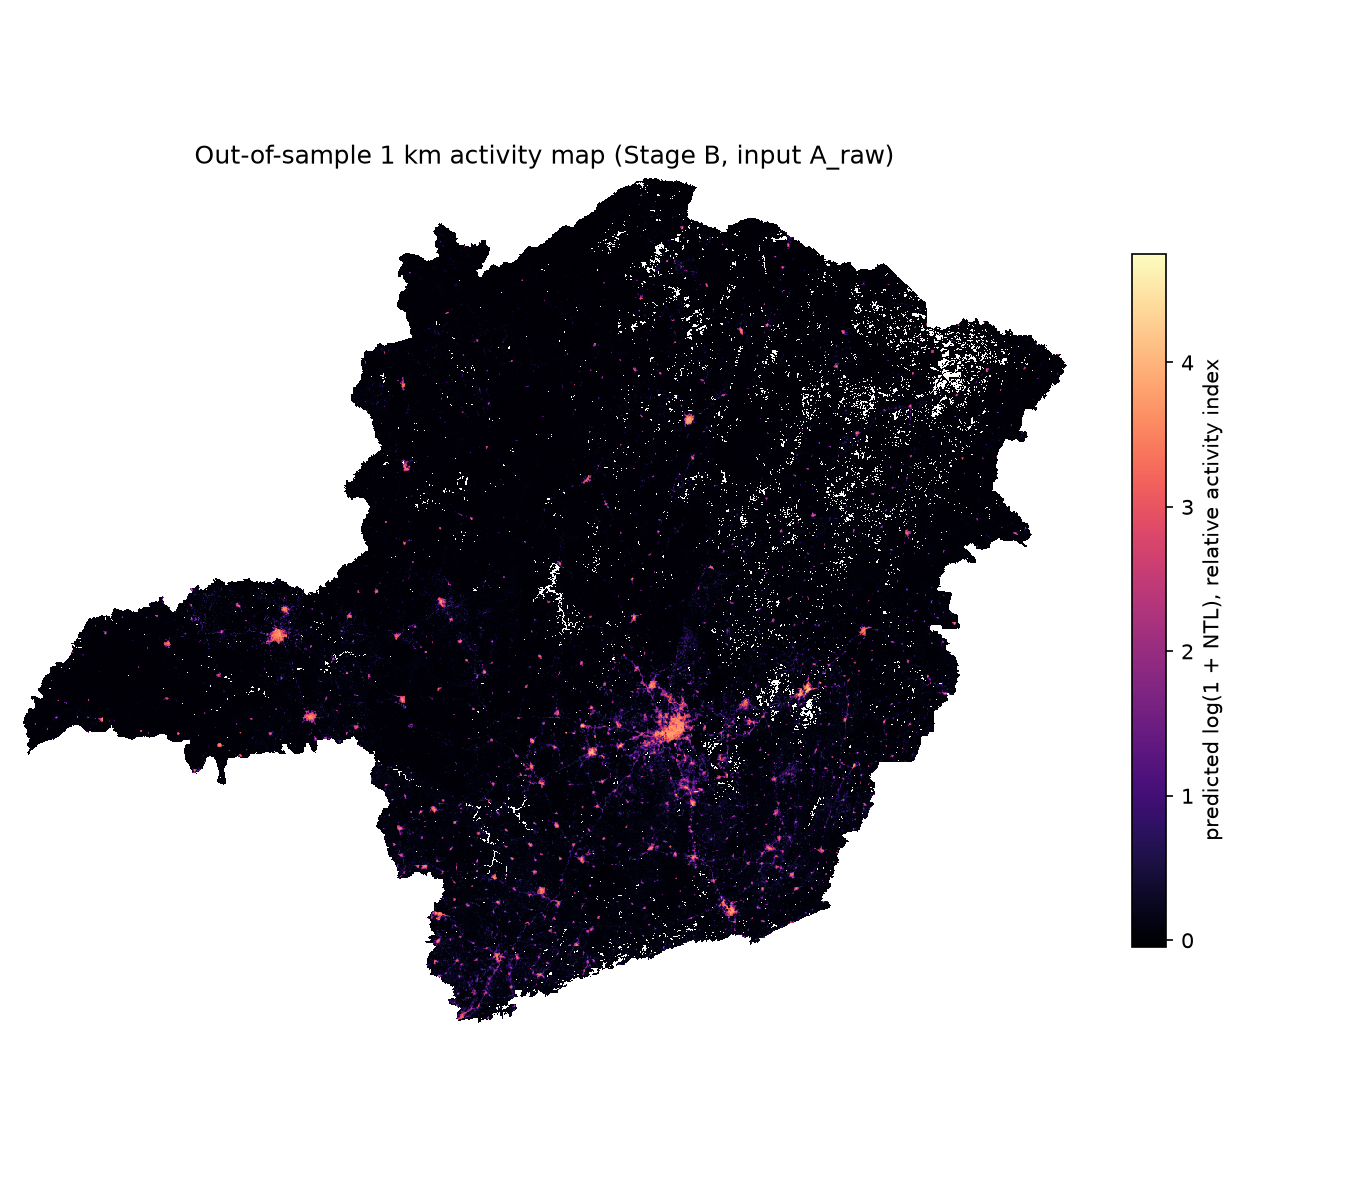
\includegraphics[width=\linewidth,trim=60 80 40 80,clip]{activity_1km.png}
\caption{Out-of-sample 1\,km activity index (Stage B).}\label{fig:activity}\end{subfigure}\hfill
\begin{subfigure}[b]{0.42\linewidth}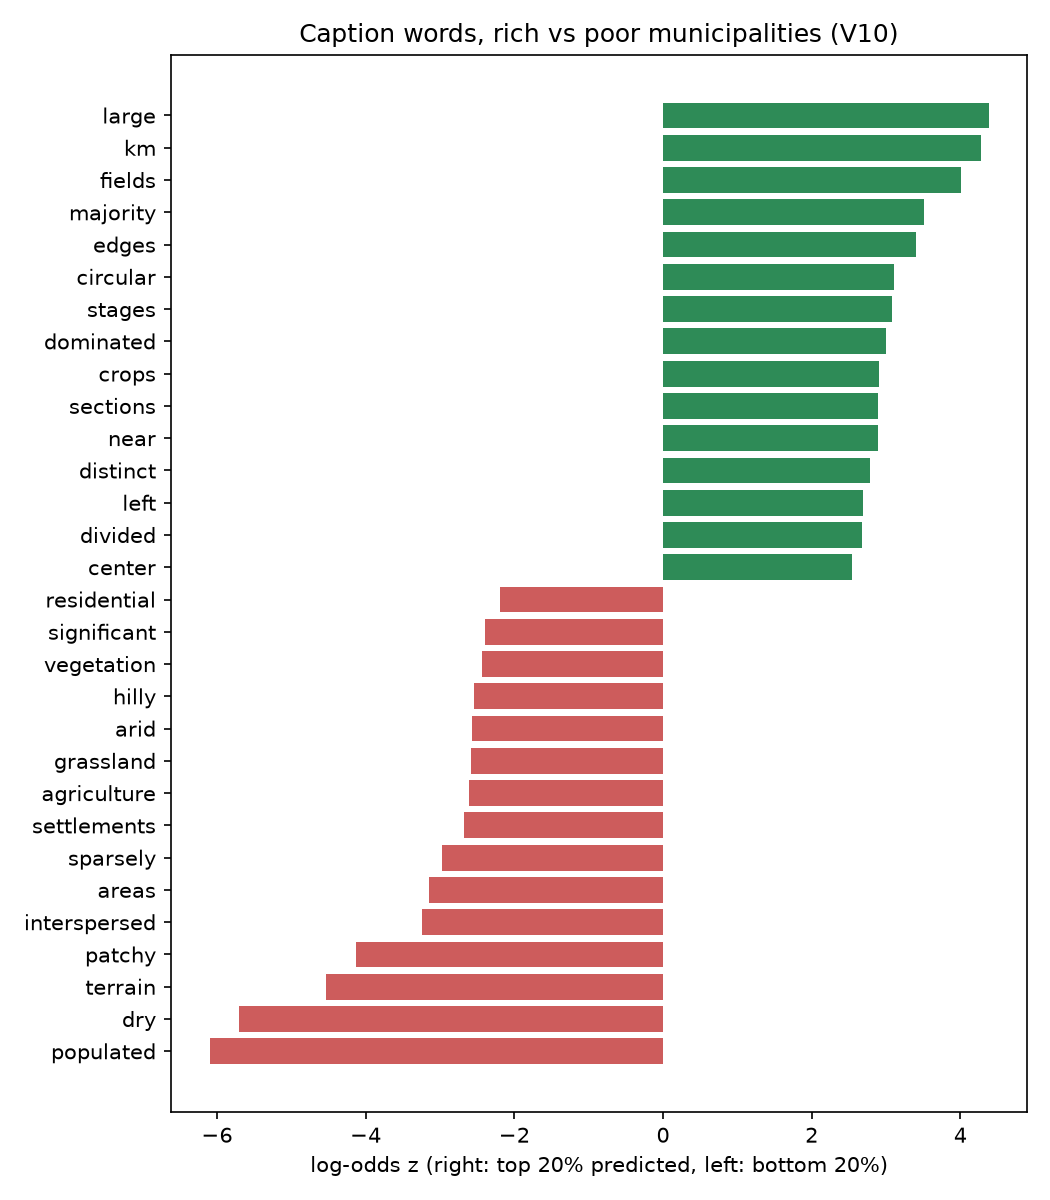
\includegraphics[width=\linewidth]{word_contrast.png}
\caption{Caption words, top vs bottom 20\% predicted.}\label{fig:words}\end{subfigure}
\caption{Cell-level output and what the captions say.}
\end{figure}

%=====================================================================
\section{What the text says}

\paragraph{Nearest captions.} For a few municipalities we list the training captions nearest to the municipality's
mean cell embedding in the Stage A space of the round where it is tested
(\texttt{reports/tables/explanations.md}). For Belo Horizonte (official 10.82, predicted 10.91) all five are dense
residential grids with red-tiled roofs and 60--74\% built-up. For the poorest municipality, São João das Missões
(8.99 vs 9.08), they describe sparse settlements in dry scrub. For Conceição do Mato Dentro, a mining town (11.94 vs
10.46), they describe forest and pasture, which is exactly why it is under-predicted: the text describes what is
visible, and the mine's value is not visible in most of the municipality's cells.

\paragraph{Rich vs poor words.} Figure~\ref{fig:words} contrasts caption words of the top and bottom 20\% of predicted
municipalities (log-odds with an informative Dirichlet prior, Monroe et al., 2008). Rich places are described with
\emph{large, fields, circular, crops, divided, sections}: mechanised agriculture with centre-pivot irrigation, the
Triângulo's agribusiness. Poor places get \emph{sparsely populated, dry, terrain, patchy, arid, hilly, settlements}.
The words are interpretable and match the economic geography of the state.

\subsection{How reliable are the captions? A blind audit}

We drew 300 captions at random and labelled each of their 1{,}801 sentences as \emph{correct}, \emph{false} (claims
something the tile contradicts) or \emph{vague} (true but says nothing specific), looking at the tile and without
seeing which sentences the cleaning had dropped. Raw and cleaned results are derived from the same labels.
\textbf{The labelling was done by an LLM (Claude, Anthropic), looking at each tile beside its sentences under fixed
written rules, not by a human annotator.} A second, human labeller for a subset (to compute Cohen's kappa) was not
available in time; the label sheet is in the repository for that purpose.

\begin{table}[!htbp]
\centering\small
\caption{Caption audit, 300 random captions (1{,}801 sentences), Wilson 95\% intervals. Labels: 1{,}440 correct, 235
vague, 126 false.}
\label{tab:audit}
\begin{tabular}{@{}lrrl@{}}
\toprule
Measure & $n$ & value & 95\% CI \\
\midrule
captions with $\geq$1 false claim, raw & 300 & 34.7\% & [29.5, 40.2] \\
captions with $\geq$1 false claim, after cleaning (captions still used) & 284 & 23.2\% & [18.7, 28.5] \\
rule-dropped sentences that were false or vague (precision) & 288 & 58.0\% & [52.2, 63.5] \\
false sentences removed by cleaning (recall) & 126 & 41.3\% & [33.1, 50.0] \\
\bottomrule
\end{tabular}
\end{table}

Only 7\% of sentences are false, but because captions have six sentences, a third of raw captions contain at least
one (Table~\ref{tab:audit}). Cleaning cuts this to 23\%. The typical false claims are: ``no buildings'' on tiles with
a few farmhouses, ``farmland'' on natural scrub or forest, ``industrial or mining activity'' on centre-pivot fields or
quarries, ``no roads'' on tiles with dirt tracks, and ponds that are not there. The cleaning removes 41\% of the false
sentences, and 58\% of what it removes is false or vague; the rest are true sentences the keyword rules
misjudged (for example ``field'' in a town with a sports field). Consistent with V8 $\approx$ V7, this level of noise
does not hurt the GDP estimate, probably because the alignment only uses text in training and the fact sentences
carry most of the reliable content.

%=====================================================================
\section{Limitations}
\begin{itemize}
\item \textbf{Frozen GSED.} Stage A and B can only reorganise the 64 GSED numbers; any gain from text comes from a
better-organised space, not new information. Fine-tuning an image encoder on the tiles was out of scope.
\item \textbf{Contrastive loss only.} UrbanCLIP's ablation found the language-modelling loss alone beat contrastive
alone; we kept only the contrastive part, as in the proposal.
\item \textbf{Audit labels.} The 300-caption audit was labelled by an LLM, not by people, and by a single labeller,
so no agreement statistic is available. LLM judgements of small features (a pond, a farmhouse) can be wrong.
\item \textbf{Revisions after the first test results.} Stage C's recalibration and grid were chosen on validation
data, but after the first test results were seen (Section 4.2).
\item \textbf{Data years and sources.} WorldCover is 2021 and sector shares are 2021; Esri imagery mixes capture dates
around 2020--2023; OSM is sparse in rural areas. IBGE publishes no data-quality indicator per municipality, so that
part of the embedding paper's error analysis could not be repeated.
\item \textbf{Hybrid.} V10 can pick a different base model in each round, so it is a procedure rather than one model.
\item \textbf{Growth extension not done.} The optional growth test (Phase 10) needs GSED and VIIRS for 2018--2021;
the Earth Engine project's monthly quota was exhausted, and the gate rule of the plan dropped it first.
\item \textbf{One state.} All results are for Minas Gerais; transfer to other states or countries is untested.
\end{itemize}

%=====================================================================
\section{Conclusion}
Free satellite data explain about half of the variation in municipal GDP per capita across Minas Gerais when tested
on regions the model never saw (\R{} 0.52 vs 0.27 for night lights alone). The gain comes mainly from learning which
1\,km cells matter (Stage C pooling) and, to a smaller degree, from aligning embeddings with text. Night-light steering,
POIs and roads, and the hybrid add nothing significant once Stage C is well calibrated, and an early ``steering
helps'' result disappeared when the aggregator was fixed, which shows how much honest spatial testing matters. The
model fails where output is concentrated and invisible: mines, steel mills and logistics hubs, together with small
commuter and public-sector towns. Generated captions are useful but noisy (a third contain a false claim), and simple
data checks remove a good part of that noise. A natural next step is to give the model information that satellites
cannot see, such as registered firms or mining licences, for the municipalities where it fails.

\paragraph{Reproducibility.} Code, configuration and all tables and figures are in the repository (tag
\texttt{v1.0-results}). \texttt{scripts/run\_all.sh} reruns every step from the raw downloads; data live outside the
repository. The release folder contains the cell feature table, the cleaned captions, the audit labels, all
predictions and the 1\,km activity GeoTIFF; Esri tiles are not redistributed.

\section*{References}
{\small
\begin{itemize}[leftmargin=*,label={}]
\item Brown, C.\,F. et al.\ (2025). AlphaEarth Foundations / Google Satellite Embedding dataset (GSED), Earth Engine.
\item Hu, Y.\ and Yao, J.\ (2022). Illuminating economic growth. \emph{Journal of Econometrics} 228(2), 359--378.
\item IBGE (2024). Produto Interno Bruto dos Municípios; Censo Demográfico 2022; Divisão Regional do Brasil 2017.
\item Monroe, B.\,L., Colaresi, M.\,P.\ and Quinn, K.\,M.\ (2008). Fightin' words. \emph{Political Analysis} 16(4), 372--403.
\item Liu, F.\ et al.\ (2024). RemoteCLIP: a vision language foundation model for remote sensing. \emph{IEEE TGRS} 62.
\item Bai, S.\ et al.\ (2025). Qwen2.5-VL technical report. arXiv:2502.13923.
\item Yan, Y.\ et al.\ (2024). UrbanCLIP: learning text-enhanced urban region profiling with contrastive language--image
pretraining from the web. \emph{Proceedings of the ACM Web Conference 2024}.
\item Yue, Zhao and Hu (2026). Estimating economic activity from satellite embeddings. \emph{Applied Sciences} 16, 582.
\item Zanaga, D.\ et al.\ (2022). ESA WorldCover 10\,m 2021 v200.
\end{itemize}}

\end{document}
